% =====================================================================
% DUNE — IEEE Robotics and Automation Practice (RA-P) submission
%
% RA-P is a short, practice-first journal. Target length: keep the body
% at/under 6 pages INCLUDING references (the four sample papers run 5-6).
% Verify the exact page limit against the current RA-P author guidelines
% before final submission.
%
% Build:  pdflatex main && bibtex main && pdflatex main && pdflatex main
% =====================================================================
\documentclass[10pt,journal,letterpaper]{IEEEtran}

\usepackage[T1]{fontenc}
\usepackage[utf8]{inputenc}
\usepackage{amsmath,amssymb,bm}
\usepackage{graphicx}
\usepackage{booktabs}
\usepackage{url}
\usepackage{xcolor}
\usepackage{siunitx}
\usepackage{tikz}
\usetikzlibrary{arrows.meta,positioning,calc,shapes.geometric,fit,backgrounds,decorations.pathreplacing}
\usepackage{pgfplots}
\pgfplotsset{compat=1.18}
\usepackage{placeins}
\usepackage[hidelinks]{hyperref}
\usepackage{cite}

% --- shared figure palette (matches text, colour-blind safe) ---
\definecolor{cBlue}{HTML}{2A6EBB}
\definecolor{cBlueL}{HTML}{DCEAF7}
\definecolor{cGreen}{HTML}{2E7D57}
\definecolor{cGreenL}{HTML}{D3ECE0}
\definecolor{cAmber}{HTML}{B5730A}
\definecolor{cAmberL}{HTML}{F6E4BE}
\definecolor{cRed}{HTML}{B23A2E}
\definecolor{cRedL}{HTML}{F5D6D1}
\definecolor{cGray}{HTML}{5B6470}
\definecolor{cGrayL}{HTML}{ECEEF1}

% --- draft aids (remove before submission) ---
\newcommand{\todo}[1]{\textcolor{red}{\textbf{[TODO: #1]}}}

% --- notation ---
\newcommand{\pvec}{\mathbf{p}}
\newcommand{\avec}{\mathbf{a}}
\newcommand{\xvec}{\mathbf{x}}

\begin{document}

\title{DUNE: A Reproducible, Low-Cost Indoor UWB\\
  Positioning Stack for Small Rovers}

\author{Adersh~Maruvattu,~Atharva~Chavan,~and~Ashish~Dutta% <-this % stops a space
\thanks{Manuscript received \todo{date}; revised \todo{date}.}%
\thanks{A.~Maruvattu and A.~Chavan contributed equally to this work.}%
\thanks{A.~Maruvattu and A.~Dutta are with the Indian Institute of
  Technology Kanpur, Kanpur, India (e-mail: adm20@iitk.ac.in;
  adutta@iitk.ac.in).}%
\thanks{A.~Chavan is with the Indian Institute of Technology Indore,
  Indore, India (e-mail: me240003021@iiti.ac.in).}%
\thanks{Code, calibration data, and logs:
  \url{https://github.com/AdershM-2/UWB_3}.}}

\markboth{IEEE Robotics and Automation Practice (RA-P), Preprint}%
{Maruvattu \MakeLowercase{\textit{et al.}}: DUNE: A Reproducible, Low-Cost Indoor UWB Positioning Stack for Small Rovers}

\maketitle

\begin{abstract}
This paper presents DUNE, an open-source indoor ultra-wideband (UWB)
positioning system for small mobile robots built from commodity
DecaWave~DW1000 transceivers. The system integrates a two-stage range
calibration that removes antenna-delay and received-power biases, a
continuous non-line-of-sight (NLOS) weighting derived from the
first-path-to-total received-power ratio, and a moving-horizon estimator
that exploits a two-tag rigid-body constraint to observe heading. Anchor
coordinates are determined automatically from inter-anchor ranging,
eliminating any external survey of the infrastructure. As the estimator
depends only on standard range and first-path-power reports, it applies
without modification to successor transceivers such as the DW3000. The
system is evaluated on a five-anchor sand-arena testbed against an
overhead-camera reference: calibration reduces the single-reading
horizontal error from \SI{199}{} to \SI{94}{\milli\meter}, temporal
filtering attains \SI{60}{}--\SI{65}{\milli\meter} at rest, the
self-survey recovers the anchor geometry to \SI{51}{\milli\meter}, and a
driven trajectory under continuous ground truth is tracked at
\SI{124}{\milli\meter} RMSE. The complete firmware, host software,
calibration data, and logs are released.

\end{abstract}

\begin{IEEEkeywords}
Ultra-wideband, indoor localization, range sensing, NLOS mitigation,
sensor fusion, calibration, reproducible robotics.
\end{IEEEkeywords}

\IEEEpeerreviewmaketitle

% ---------------------------------------------------------------
% FIG 1 — system pipeline (native TikZ, full width)
% ---------------------------------------------------------------
\begin{figure*}[t]
  \centering
  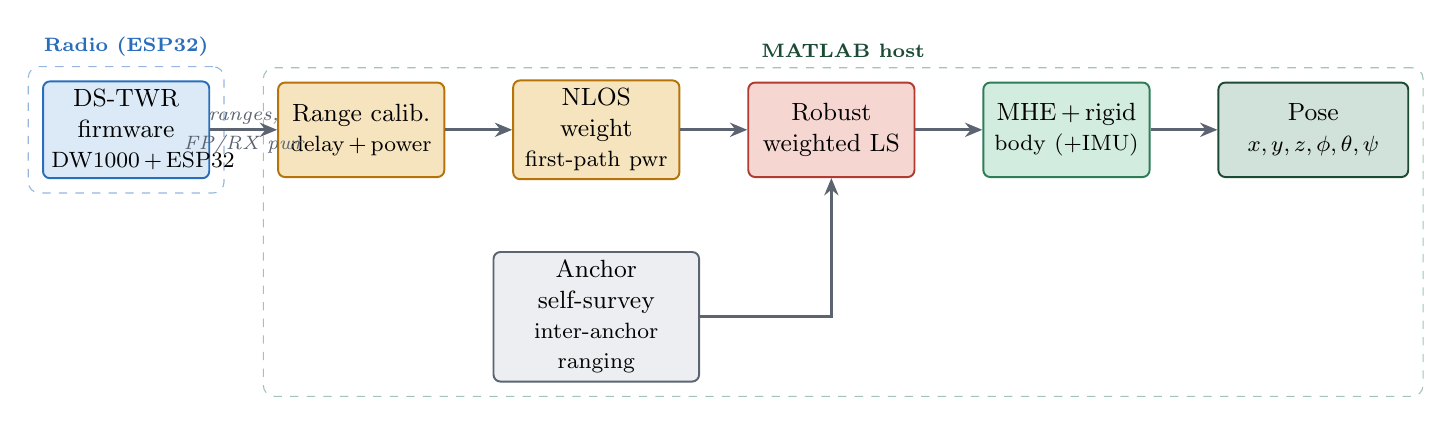
\begin{tikzpicture}[
    font=\small,
    >={Stealth[length=2.2mm,width=1.8mm]},
    blk/.style={rectangle, rounded corners=2.5pt, draw, line width=0.7pt,
      minimum height=12mm, text width=19mm, align=center, inner sep=3pt},
    flow/.style={-{Stealth[length=2.2mm,width=1.8mm]}, line width=1pt, draw=cGray},
    lbl/.style={font=\scriptsize\itshape, text=cGray, inner sep=1.5pt},
    node distance=8mm and 8.5mm]

    \node[blk, draw=cBlue,  fill=cBlueL]  (fw)   {DS-TWR firmware\\ \footnotesize DW1000\,+\,ESP32};
    \node[blk, draw=cAmber, fill=cAmberL, right=of fw]   (cal)  {Range calib.\\ \footnotesize delay\,+\,power};
    \node[blk, draw=cAmber, fill=cAmberL, right=of cal]  (nlos) {NLOS weight\\ \footnotesize first-path pwr};
    \node[blk, draw=cRed,   fill=cRedL,   right=of nlos] (fix)  {Robust\\ weighted LS};
    \node[blk, draw=cGreen, fill=cGreenL, right=of fix]  (est)  {MHE\,+\,rigid\\ \footnotesize body ($+$IMU)};
    \node[blk, draw=cGreen!60!black, fill=cGreen!22, right=of est, text width=22mm]
      (pose) {Pose\\ \footnotesize $x,y,z,\phi,\theta,\psi$};

    \node[blk, draw=cGray, fill=cGrayL, below=9mm of nlos, text width=24mm]
      (surv) {Anchor self-survey \\ \footnotesize inter-anchor ranging};

    \draw[flow] (fw)   -- node[lbl,above]{ranges,} node[lbl,below]{FP/RX pwr}  (cal);
    \draw[flow] (cal)  -- (nlos);
    \draw[flow] (nlos) -- (fix);
    \draw[flow] (fix)  -- (est);
    \draw[flow] (est)  -- (pose);
    \draw[flow] (surv.east) -| (fix.south);

    \begin{scope}[on background layer]
      \node[draw=cBlue!50, dashed, rounded corners, inner sep=5pt,
        fit=(fw), label={[cBlue,font=\scriptsize\bfseries]above:Radio (ESP32)}] {};
      \node[draw=cGreen!45, dashed, rounded corners, inner sep=5pt,
        fit=(cal)(pose)(surv),
        label={[cGreen!60!black,font=\scriptsize\bfseries]above:MATLAB host}] {};
    \end{scope}
  \end{tikzpicture}
  \caption{The DUNE pipeline. Five DW1000 anchors and one or two ESP32
  tags perform double-sided two-way ranging; the host calibrates each
  range for antenna delay and received-power bias, weights it by a
  first-path NLOS score, solves a robust least-squares fix, and fuses
  the stream in a moving-horizon estimator with a two-tag rigid-body
  constraint. Anchor coordinates are supplied by an inter-anchor
  self-survey, and roll, pitch, and height are read from the on-board
  IMU to complete the six-degree-of-freedom pose.}
  \label{fig:pipeline}
\end{figure*}

\section{Introduction}
\label{sec:intro}

\IEEEPARstart{A}{ccurate} indoor localization is a prerequisite for
autonomous mobile robots operating where satellite navigation is
unavailable. Among the candidate technologies, ultra-wideband (UWB)
ranging offers a favourable combination of centimetre-level time-of-flight
resolution, robustness to multipath relative to narrowband radio, and
low unit cost, and it has become a common choice for real-time
localization systems~\cite{alarifi2016uwb}. A single DW1000 transceiver
can time a radio round trip to a few centimetres, and the underlying
two-way ranging and multilateration are well established~\cite{dstwr_neirynck}.

In practice, however, a substantial gap separates this nominal ranging
resolution from the pose accuracy a robot experiences during operation.
Raw transceiver ranges carry hardware- and signal-dependent biases of
several decimetres; obstructed, non-line-of-sight (NLOS) paths inflate
the measured distance without any external indication; and the anchor
coordinates that anchor the whole solution must themselves be obtained,
conventionally by manual survey or an external camera on which the
deployment then depends. Closing this gap is largely a matter of
engineering that is seldom reported in reproducible detail, so each new
deployment tends to repeat it.

This paper documents a complete, low-cost UWB positioning stack, DUNE,
that addresses these issues end to end and is released in full. The
system localizes a small Ackermann rover from five fixed DW1000 anchors
and one or two ESP32-hosted tags, with all estimation performed on a
host computer (Fig.~\ref{fig:pipeline}). The design targets
reproducibility on commodity hardware rather than a single algorithmic
novelty, and its accuracy derives from the disciplined combination of
calibration, NLOS-aware estimation, and automatic infrastructure
localization described in the following sections.

The main contributions are:
\begin{enumerate}
  \item A complete and openly released pipeline from raw double-sided
  two-way ranging to a filtered vehicle pose, including a two-step radio
  calibration (antenna delay and received-power range bias). Unlike
  common open DW1000 libraries, which target a fixed small anchor set,
  the pipeline supports an arbitrary number of anchors ($N\!\ge\!4$) and
  degrades gracefully when only a subset responds.
  \item A continuous first-path-power NLOS weighting integrated with a
  robust weighted least-squares solver and a moving-horizon estimator
  that enforces a two-tag rigid-body constraint to recover heading.
  \item An automatic anchor self-localization procedure that recovers
  the anchor geometry from inter-anchor ranging alone, eliminating the
  need for an external survey of the infrastructure.
\end{enumerate}

\section{Related Work}
\label{sec:related}

\subsection{UWB positioning and NLOS mitigation}
UWB indoor positioning has been studied extensively; a comprehensive
survey is given in~\cite{alarifi2016uwb}. Fully open systems remain
comparatively rare: ATLAS provides an open time-difference-of-arrival
localizer~\cite{tiemann2017atlas}, and the UTIL dataset~\cite{zhao2024util}
releases labelled ranging logs for benchmarking. A dominant error source
in cluttered environments is non-line-of-sight propagation, in which an
obstructed direct path forces the signal along a longer route and biases
the range positively. Kolakowski and Modelski~\cite{kolakowski2017nlos}
mitigate this by classifying each link as line-of-sight or NLOS from the
DW1000 first-path power and feeding the decision to an extended Kalman
filter. Rather than a hard classification, we derive a continuous weight
from the first-path-to-total power ratio measured within the same range
report, which both attenuates suspect ranges in the position solve and
inflates their variance in the temporal filter.

\subsection{Anchor self-calibration}
The anchor coordinates required by any multilateration system are
conventionally measured by hand or with external instrumentation.
Self-calibration methods that instead infer the anchor layout from radio
measurements are surveyed in~\cite{ridolfi2021selfcal}. Recent work
scales anchor calibration to large environments using Gaussian
processes, but relies on a LiDAR-inertial odometry trajectory as
input~\cite{yuan2025uwbgp}. In contrast, the self-survey used here
requires only the pairwise ranges the anchors can already measure among
themselves, and recovers the constellation by classical multidimensional
scaling~\cite{torgerson1952mds}.

\section{Problem Definition}
\label{sec:problem}

Consider a set of $N\!\ge\!4$ fixed anchors with positions
$\{\avec_k\}_{k=1}^{N}\subset\mathbb{R}^3$ expressed in a common world
frame. A rover carries $M\in\{1,2\}$ tags on a rigid plate; for $M{=}2$
the two tag antennas are separated by a known baseline $L$. The rover
motion is planar, so its configuration is the body pose
$\xvec=(c_x,c_y,\psi)\in SE(2)$---planar position $\mathbf{c}$ and
heading $\psi$---which is extended to the full six-degree-of-freedom
pose using the height $z$ and the roll and pitch $(\phi,\theta)$ read
from the on-board IMU. The two tag positions follow from the body pose
as
\begin{equation}
  \pvec_{1,2} = \mathbf{c} \pm \tfrac{L}{2}\,[\cos\psi,\ \sin\psi]^{\!\top},
  \label{eq:rigid}
\end{equation}
for the front and rear tag respectively.

Each double-sided two-way ranging exchange between tag $i$ and anchor
$k$ produces a range estimate that departs from the true geometric
distance by several additive terms,
\begin{equation}
  \rho_{ik} = \lVert \pvec_i - \avec_k \rVert
            + \delta_k + \gamma_k(P_{ik}) + \Delta_{ik} + \varepsilon_{ik},
  \label{eq:measmodel}
\end{equation}
where $\delta_k$ is the per-anchor antenna-delay bias, $\gamma_k(P_{ik})$
a bias that depends on the received power $P_{ik}$, $\Delta_{ik}\ge 0$
the excess path length introduced under NLOS conditions, and
$\varepsilon_{ik}\sim\mathcal{N}(0,\sigma^2)$ zero-mean measurement
noise. The tags report at different instants, so the ranges arrive
asynchronously rather than as synchronized snapshots.

The problem is twofold. First, given the anchor positions and a stream
of asynchronous ranges~\eqref{eq:measmodel}, estimate the body
trajectory $\{\xvec_t\}$ online at the sensor rate ($\ge\!5$\,Hz) while
suppressing the systematic biases and NLOS excess. Second, when the
anchor positions are not externally available, estimate
$\{\avec_k\}$ from inter-anchor ranging alone. The remainder of the
paper addresses these two problems and evaluates the resulting accuracy
against an independent optical ground truth.

\section{Methodology}
\label{sec:method}

\subsection{Ranging and range calibration}
Each range is obtained by a double-sided two-way exchange (DS-TWR),
whose symmetric four-timestamp formulation cancels the clock-frequency
offset between the two uncoordinated crystals to first
order~\cite{dstwr_neirynck} (Fig.~\ref{fig:dstwr}). One DW1000 timer
tick corresponds to \SI{4.69}{\milli\meter} of range and sets the
resolution of every calibration constant below. The two systematic
biases in~\eqref{eq:measmodel} are removed in sequence. The
antenna-delay term $\delta_k$, which reflects the propagation time
internal to each board, is calibrated per anchor against a reference
position and stored on the device, after which all anchors agree with
the reference distance to within $\pm\SI{16}{\milli\meter}$. The
residual power-dependent bias $\gamma_k$ is modelled per anchor as an
affine function of the first-path power $P_{\mathrm{fp}}$, which is more
stable than total power,
\begin{equation}
  \hat{d}_k = \rho_k - \big(a_k\,P_{\mathrm{fp},k} + b_k\big),
  \qquad a_k\in[7.7,\,9.5]\ \si{\milli\meter\per\dB},
  \label{eq:power}
\end{equation}
with $P_{\mathrm{fp}}$ clamped to the fitted interval so that the model
is never extrapolated. The coefficients are estimated once by
leave-one-position-out regression over a static campaign.

\begin{figure}[t]
  \centering
  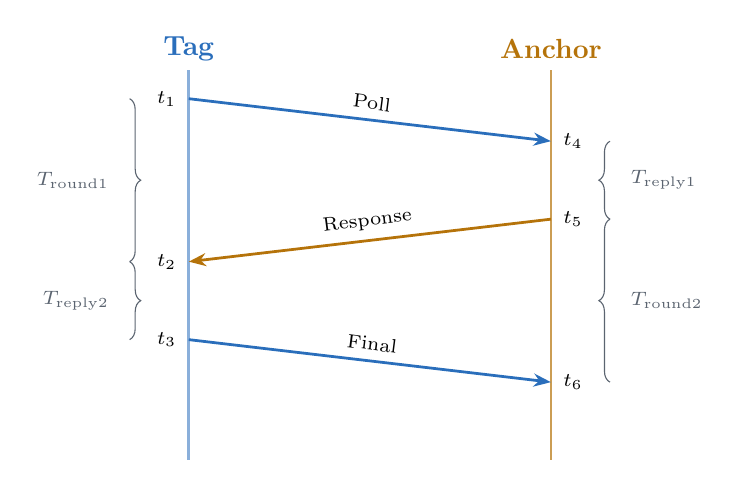
\begin{tikzpicture}[font=\small, >={Stealth[length=2.2mm]}, yscale=0.9]
    \node[font=\bfseries, text=cBlue]  at (0,0.4)  {Tag};
    \node[font=\bfseries, text=cAmber] at (4.6,0.4){Anchor};
    \draw[cBlue!55, line width=1pt]  (0,0.1)   -- (0,-5.4);
    \draw[cAmber!70, line width=1pt] (4.6,0.1) -- (4.6,-5.4);
    \draw[->, line width=1pt, draw=cBlue]  (0,-0.3)  -- node[above,sloped,font=\scriptsize]{Poll}     (4.6,-0.9);
    \draw[->, line width=1pt, draw=cAmber] (4.6,-2.0) -- node[above,sloped,font=\scriptsize]{Response} (0,-2.6);
    \draw[->, line width=1pt, draw=cBlue]  (0,-3.7)  -- node[above,sloped,font=\scriptsize]{Final}    (4.6,-4.3);
    \foreach \y/\t in {-0.3/t_1, -2.6/t_2, -3.7/t_3} \node[left=1pt,font=\scriptsize] at (0,\y) {$\t$};
    \foreach \y/\t in {-0.9/t_4, -2.0/t_5, -4.3/t_6} \node[right=1pt,font=\scriptsize] at (4.6,\y) {$\t$};
    \draw[decorate,decoration={brace,amplitude=4pt},cGray]
      (-0.75,-0.3) -- node[left=4pt,font=\scriptsize]{$T_{\mathrm{round}1}$} (-0.75,-2.6);
    \draw[decorate,decoration={brace,amplitude=4pt},cGray]
      (-0.75,-2.6) -- node[left=4pt,font=\scriptsize]{$T_{\mathrm{reply}2}$} (-0.75,-3.7);
    \draw[decorate,decoration={brace,amplitude=4pt,mirror},cGray]
      (5.35,-0.9) -- node[right=4pt,font=\scriptsize]{$T_{\mathrm{reply}1}$} (5.35,-2.0);
    \draw[decorate,decoration={brace,amplitude=4pt,mirror},cGray]
      (5.35,-2.0) -- node[right=4pt,font=\scriptsize]{$T_{\mathrm{round}2}$} (5.35,-4.3);
  \end{tikzpicture}
  \caption{Double-sided two-way ranging. Four host-side timestamps over
  two round trips recover the time-of-flight without a shared clock; the
  symmetric form is first-order insensitive to crystal frequency offset.}
  \label{fig:dstwr}
\end{figure}

\subsection{Robust NLOS-aware estimation}
Under obstruction the first signal component is attenuated relative to
the total received energy, so the gap between total and first-path power
is a direct indicator of the NLOS excess $\Delta_{ik}$
(Fig.~\ref{fig:nlos}). Denoting this gap $g_k = P_{\mathrm{rx},k} -
P_{\mathrm{fp},k}$ in decibels, each range is assigned a continuous
weight
\begin{equation}
  w_k = \max\!\Big(w_{\mathrm{f}},\ 10^{-\max(0,\,g_k-\tau)/10}\Big),
  \label{eq:nlos}
\end{equation}
with LOS threshold $\tau=\SI{3}{\dB}$ and floor $w_{\mathrm{f}}=0.05$:
below the threshold a range keeps unit weight, above it the weight decays
with the excess gap, and the floor prevents any single anchor from being
discarded outright. The instantaneous fix follows from robust weighted
multilateration,
\begin{equation}
  \pvec^\star = \arg\min_{\pvec}\;
  \sum_{k=1}^{N} w_k\,\rho_\delta\!\big(\lVert \pvec-\avec_k\rVert - \hat{d}_k\big),
  \label{eq:ls}
\end{equation}
where $\rho_\delta$ is the Huber loss and a $\chi^2$ consistency gate
rejects gross outliers, so that an inconsistent range bends rather than
dominates the solution.

The trajectory itself is estimated by a moving-horizon estimator (MHE)
that, at each step, jointly optimizes the last $N_{\mathrm{h}}$ states
($N_{\mathrm{h}}{=}10$, $\approx\!\SI{2}{\second}$) so that new evidence
can revise the recent estimate:
\begin{equation}
\begin{aligned}
  \min_{\{\xvec_k\}}\ &
  \sum_{k}\sum_{j} w_{kj}\,\rho_\delta\!\big(\lVert\pvec_k-\avec_j\rVert - \hat{d}_{kj}\big)\\[-1pt]
  &{}+ \sum_{k}\big\lVert \xvec_{k+1}-f(\xvec_k)\big\rVert^2_{Q^{-1}}
  + \big\lVert \xvec_1-\bar{\xvec}\big\rVert^2_{P^{-1}},
\end{aligned}
\label{eq:mhe}
\end{equation}
where the first term fits every windowed range under the same weighted
robust loss, the second penalizes departures from the kinematic motion
model $f(\cdot)$, and the third is an arrival cost coupling the window to
the previous estimate. The same weights $w_{kj}$ scale the measurement
variances, so the NLOS score governs both the fix and the filter. The
IMU contributes only differential quantities---yaw rate and
gravity-referenced roll and pitch---never an absolute heading; because
the Ackermann platform cannot slip laterally, $f(\cdot)$ constrains the
body velocity to the heading direction. For two tags, the rigid
constraint~\eqref{eq:rigid} is imposed by construction, so a single body
state generates both tag predictions, the baseline is exact in every
solution, and the heading is observed directly by the radios with a
per-reading resolution $\sigma_\psi \approx \sqrt{2}\,\sigma_d/L$
($\approx\!4.6^\circ$ for $\sigma_d\!=\!30$\,mm, $L\!=\!0.527$\,m),
further reduced by filtering.

\begin{figure}[t]
  \centering
  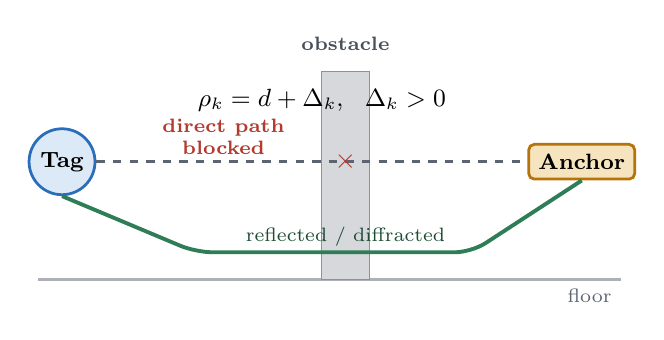
\begin{tikzpicture}[font=\small, >={Stealth[length=2.2mm]}]
    \draw[cGray!50, line width=1pt] (-0.3,-1.5) -- (7.1,-1.5);
    \node[cGray, font=\scriptsize] at (6.7,-1.7) {floor};
    \fill[cGray!25, draw=cGray!70] (3.3,-1.5) rectangle (3.9,1.15);
    \node[cGray!80!black, font=\scriptsize\bfseries, align=center] at (3.6,1.5) {obstacle};
    \node[circle, draw=cBlue, fill=cBlueL, line width=1pt, inner sep=2.5pt]
      (tag) at (0,0) {\footnotesize\bfseries Tag};
    \node[rectangle, rounded corners=2pt, draw=cAmber, fill=cAmberL,
      line width=1pt, inner sep=3.5pt] (anc) at (6.6,0) {\footnotesize\bfseries Anchor};
    \draw[dashed, cGray, line width=1pt] (tag) -- (anc);
    \node[cRed, font=\bfseries] at (3.6,0) {$\times$};
    \node[cRed, font=\scriptsize\bfseries, align=center] at (2.05,0.32) {direct path\\ blocked};
    \draw[cGreen, line width=1.4pt, rounded corners=6pt]
      (tag.south) -- (1.7,-1.15) -- (3.6,-1.15) -- (5.2,-1.15) -- (anc.south);
    \node[cGreen!60!black, font=\scriptsize] at (3.6,-0.95) {reflected / diffracted};
    \node[align=center, font=\small] at (3.3,0.78) {$\rho_k = d + \Delta_k,\ \ \Delta_k>0$};
  \end{tikzpicture}
  \caption{NLOS mechanism. When the direct path is obstructed the signal
  reaches the anchor along a longer reflected or diffracted route, so the
  measured range is biased positively by $\Delta_k$. The bias is
  estimated from the total-to-first-path power gap and used to weight the
  range through~\eqref{eq:nlos}.}
  \label{fig:nlos}
\end{figure}

\subsection{Automatic anchor localization}
When the anchor coordinates are not measured externally, they are
recovered from the ten pairwise inter-anchor ranges of the five-anchor
set. A set of mutual distances defines a rigid configuration up to an
isometry, and classical multidimensional scaling~\cite{torgerson1952mds}
returns the point set whose pairwise distances best match the measured
ranges. The triggering tag only relays messages, so its own antenna
delay does not enter the survey. The recovered constellation is
determined up to a rotation and reflection, resolved against a single
known landmark or, for evaluation, aligned to a reference layout without
scaling.

\section{Experimental Results}
\label{sec:results}

The system was evaluated in a sand-filled arena with five DW1000
anchors---four at ground level near the corners and one elevated---whose
coordinates were fixed either by the self-survey of
Section~\ref{sec:method} or by an overhead camera. The rover carried a
front and a rear tag separated by $L=\SI{0.527}{\meter}$, the rear tag
additionally equipped with a BNO085 IMU, together with an AprilTag
fiducial facing the ceiling. A ceiling-mounted Kinect~v2 tracked the
fiducial for ground truth; after intrinsic calibration and clicked-point
registration to the anchor frame the registration residual was
\SI{13.5}{\milli\meter}, and the marker lever arm was compensated per
sample. All estimation was performed off-board.

\subsection{Static accuracy and calibration}
Localization accuracy was first characterized with the rover stationary
at 19 surveyed positions across the arena ($\sim\!\SI{20}{\second}$ per
position, $\sim\!7\,600$ ranges). Table~\ref{tab:static} reports the
single-reading horizontal error under the two calibration stages.
Antenna-delay calibration alone leaves a floor-wide RMSE of
\SI{199}{\milli\meter}; adding the received-power correction
of~\eqref{eq:power} reduces it to \SI{94}{\milli\meter}
(Fig.~\ref{fig:calib}), the single largest improvement in the pipeline.

To quantify how much of the remaining error is irreducible by any static
correction, we evaluated an oracle that subtracts, from each position,
the mean residual measured there---the best achievable by any
time-invariant, position-dependent correction. Its residual RMSE is
\SI{72}{\milli\meter}, which therefore lower-bounds any fixed calibration
and shows that the leftover error is not a static spatial map that a
denser survey could remove. Temporal filtering nonetheless attains
\SI{60}{}--\SI{65}{\milli\meter} at rest, below this bound, because it
averages the zero-mean high-frequency component of the residual over
successive readings, leaving only a slowly varying multipath term that
the static oracle cannot capture.

\begin{table}[t]
  \centering
  \caption{Static single-reading horizontal error over 19 positions.}
  \label{tab:static}
  \begin{tabular}{@{}lccc@{}}
    \toprule
     & \textbf{RMSE} & \textbf{Median} & \textbf{95th pct.}\\
    \midrule
    Antenna-delay calibration only          & 199 & 132 & 393\\
    \;+ received-power correction            & \textbf{94} & \textbf{69} & 160\\
    Oracle (per-position constant)           & 72  & 31  & ---\\
    \bottomrule
  \end{tabular}\\[2pt]
  {\footnotesize All values in \si{\milli\meter}.}
\end{table}

\begin{figure}[t]
  \centering
  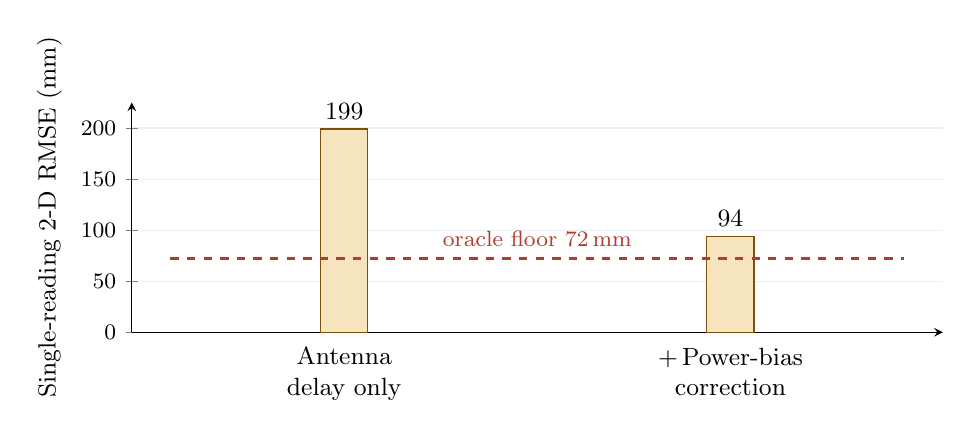
\begin{tikzpicture}
    \begin{axis}[
      width=0.98\columnwidth, height=4.5cm,
      ybar, bar width=17pt,
      ymin=0, ymax=225, xmin=0.45, xmax=2.55,
      ylabel={Single-reading 2-D RMSE (\si{\milli\meter})},
      ylabel style={font=\small},
      xtick={1,2},
      xticklabels={{Antenna\\delay only}, {+\,Power-bias\\correction}},
      xtick style={draw=none},
      x tick label style={font=\small, align=center},
      ytick={0,50,...,200}, tick label style={font=\footnotesize},
      ymajorgrids, grid style={cGrayL}, axis lines=left,
      nodes near coords, nodes near coords style={font=\small\bfseries},
      every node near coord/.append style={/pgf/number format/precision=0,
        /pgf/number format/fixed},
    ]
      \addplot[draw=cAmber!70!black, fill=cAmberL] coordinates {(1,199) (2,94)};
      \draw[dashed, cRed, line width=0.9pt] (axis cs:0.55,72) -- (axis cs:2.45,72);
      \node[font=\footnotesize, text=cRed, anchor=south] at (axis cs:1.5,74)
        {oracle floor \SI{72}{\milli\meter}};
    \end{axis}
  \end{tikzpicture}
  \caption{Effect of the two-step calibration on floor-wide single-reading
  error. The received-power correction removes the strength-dependent
  residual left by antenna-delay calibration; the dashed line marks the
  \SI{72}{\milli\meter} oracle floor of any fixed correction.}
  \label{fig:calib}
\end{figure}

\subsection{Estimator comparison and anchor self-survey}
Table~\ref{tab:est} compares the moving-horizon estimator with an
extended Kalman filter on identical recorded ranges. While the vehicle is
moving, the MHE reduces trajectory jerk by \SI{40}{}--\SI{44}{\percent}
(from 0.61 to \SI{0.36}{\meter\per\second\cubed}) for only
\SI{6}{\milli\meter} of additional lag, and the two estimators are
equivalent at rest; each MHE solve completes in \SI{3}{\milli\second},
within the \SI{6}{\hertz} update budget. The reduced jerk reflects the
window optimization rejecting isolated range excursions that a
single-step filter propagates.

The anchor self-survey was evaluated against the independently registered
overhead-camera layout (Table~\ref{tab:survey}). The raw inter-anchor
ranges are biased long by up to \SI{202}{\milli\meter}
(RMS \SI{118}{\milli\meter}) because each measurement carries the antenna
delays of both participating anchors. After multidimensional scaling and
alignment without scaling, the reconstructed constellation agrees with
the camera layout to \SI{51}{\milli\meter} RMS once the per-anchor delay
bias is removed---an independent confirmation of the geometry to within
centimetres. The deployed configuration is built from this self-survey.

\begin{table}[t]
  \centering
  \caption{Moving-horizon estimator versus Kalman filter (same logs).}
  \label{tab:est}
  \begin{tabular}{@{}lcc@{}}
    \toprule
    \textbf{Metric} & \textbf{Kalman (EKF)} & \textbf{MHE}\\
    \midrule
    Trajectory jerk, moving (\si{\meter\per\second\cubed}) & 0.61 & \textbf{0.36}\\
    Additional lag (\si{\milli\meter})       & ---  & 6\\
    RMSE at rest (\si{\milli\meter})         & 64   & \textbf{61}\\
    Solve time (\si{\milli\second})          & $<1$ & 3\\
    \bottomrule
  \end{tabular}
\end{table}

\begin{table}[t]
  \centering
  \caption{Anchor self-survey versus overhead-camera layout.}
  \label{tab:survey}
  \begin{tabular}{@{}lc@{}}
    \toprule
    \textbf{Quantity} & \textbf{Value (\si{\milli\meter})}\\
    \midrule
    Raw inter-anchor range bias (max)          & 202\\
    Raw inter-anchor range bias (RMS)          & 118\\
    Reconstructed geometry vs.\ camera (RMS)   & \textbf{51}\\
    \bottomrule
  \end{tabular}
\end{table}

\subsection{Trajectory tracking}
The full system was finally evaluated on a driven run under continuous
optical ground truth. Over the trajectory the Kinect provided 133 valid
pose samples at near-continuous coverage, and both
tags were serviced evenly (355 and 362 sweeps) with an average of five
anchors per sweep, so the ground truth constrains the entire path rather
than isolated segments. The rigid-body MHE track follows the reference
with a horizontal RMSE of \SI{124}{\milli\meter}; the estimated path
length is $1.4\times$ that of the truth, indicating that the residual is
dominated by high-frequency wander rather than a systematic offset, as
the two trajectories share the same overall shape. This moving accuracy
is consistent with the single-reading static scatter accumulating under
motion, and is limited by per-sweep range noise, which longer averaging
windows trade against lag; reducing it further through tighter range
gating and higher sweep rates is the subject of ongoing work.

\section{Conclusion}
\label{sec:conclusion}

We presented DUNE, a complete and openly released indoor UWB positioning
stack for a small mobile robot. Its accuracy follows from a two-step
range calibration, a continuous first-path-power NLOS weighting, and a
moving-horizon estimator with a two-tag rigid-body constraint, while the
anchor geometry is obtained automatically from inter-anchor ranging
rather than external survey. The system achieves a filtered static
accuracy of \SI{60}{}--\SI{65}{\milli\meter} and reconstructs the anchor
layout to \SI{51}{\milli\meter} of an optical reference. Because it
operates only on standard range and first-path-power reports, the
pipeline transfers without modification to newer transceivers such as the
DW3000. Ongoing work addresses the moving-accuracy gap through tighter
range gating and higher sweep rates. All firmware, host software,
calibration data, and logs are released to support reproduction and
extension.

\section{Implementation and Reproducibility}
\label{sec:impl}

The complete system is released at
\url{https://github.com/AdershM-2/UWB_3}. The host stack is a MATLAB
package (\texttt{+dune}) with supporting scripts
(Table~\ref{tab:sw}); the firmware comprises three Arduino sketches for
the anchor and the two tag variants. The ingest layer is
protocol-agnostic---a sweep is a set of (anchor,\,range,\,quality)
samples---so the estimators consume live serial data and replayed logs
identically, and estimation is kept out of the real-time driving loop,
which only records. The two calibration files that reproduce the accuracy
are \texttt{delay\_calibration.json} (per-anchor antenna delays, in
\SI{4.69}{\milli\meter} ticks) and \texttt{range\_correction.json}
(the per-anchor first-path-power coefficients of~\eqref{eq:power}); both
load automatically in \texttt{solveSweep}. The static-campaign readings,
driven-run recordings, and an extended engineering report are released
alongside the code.

\begin{table}[t]
  \centering
  \caption{Key released software modules.}
  \label{tab:sw}
  \footnotesize
  \begin{tabular}{@{}lp{4.7cm}@{}}
    \toprule
    \textbf{Module} & \textbf{Function}\\
    \midrule
    \texttt{Anchor.ino}, \texttt{Tag*.ino} & DW1000 DS-TWR firmware
      (anchor and two tag variants).\\
    \texttt{+dune/solveSweep}       & Calibrate, weight, and solve one sweep.\\
    \texttt{+dune/multilaterate}    & Robust weighted least-squares solver,~\eqref{eq:ls}.\\
    \texttt{+dune/gapWeights}       & First-path-power NLOS weights,~\eqref{eq:nlos}.\\
    \texttt{+dune/MheEstimator}     & Moving-horizon estimator (CasADi/IPOPT),~\eqref{eq:mhe}.\\
    \texttt{+dune/MheRigid}         & Two-tag rigid-body estimator.\\
    \texttt{tune\_delays\_sweep.m}  & Over-the-air antenna-delay calibration.\\
    \texttt{survey\_reconstruct.m}  & Multidimensional-scaling anchor self-survey.\\
    \texttt{rover\_run\_report.m}   & Driven-run scoring against Kinect truth.\\
    \bottomrule
  \end{tabular}
\end{table}


\bibliographystyle{IEEEtran}
\bibliography{refs}

\end{document}
